\chapter{Supervised learning: classificaton, regression, nearest neighbours}
\label{ch:supervised-learning}

regression = supervised learning for quantitative data.

$x->y$

if we want to classify pictures between cats and dogs, two kinds of methods:
- supervised: give information before
- unsupervised: you figure out that there are two categories, understand that
there are two categories, and learn from that.

fig 5

distincition on the nature of the variable that we want to predict.
quantitative data : why is it a real number or a vector?

we are going to see today classification. so far we've seen just supervised
quantitative : regression. there are more task to do.

today : classification.
next course : clustering.
after that : neural networks, that can be used for any of those tasks, that
involve a bit more methodology.


\section{Classification}

Let's start with a set of training data indexed with $i$:  $(x_i,k_i)$ where the
label $k_i$ can vary from 1 to $K$: $k_i = 1, 2, \ldots K$.

Again, we face a challenge in using large datasets:
\begin{equation}
    x_{N+1} \xrightarrow{?} k_{N+1}
\end{equation}

Until now, we have only used regression methods. Let's try to do the same.

\subsection{Regressions methods at one dimension}

Let's start with only two categories : $K=2$
\begin{equation}
    k_i \in \{ 0, 1 \}
\end{equation}

From these data, we can try to predict the value of K with unsupervised learning
methods. It means that we would get a classification, by trying to find how
close the data are from $0$ or $1$.

If we start with the $p=1$ case, we can represent a set of data on graph
\ref{supvlearn6}.

\begin{figure}
    \TODO
    \caption{Representation of a dataset with blue dots indexed as 0 and red
        dots indexed as 1. A linear regression can be plotted on these data
    }
    \label{supvlearn6}
\end{figure}

Here we need to find a value $x_h$ somewhere to be able to split the value
between two sets of data. Generally, we would work with more complicated
problems, in larger dimensions.

Here, if we carry out the following linear regression:

\begin{equation}
    y = \hat \alpha + \hat \beta x
\end{equation}

This is actually exactly what we did in the first lecture: we had to compute
the $\hat \alpha$ and $\hat \beta$ that gave us the best results.

The linear regression equation we get on this problem allow us to find the
decision boundary, defined as the $\hat x$ corresponding to $\hat y = \half$.
Thus, we may claim that when $\hat y$ is larger than $\half$, then $\hat k =1$,
and when it is lower than $\half$, $\hat k$ vanishes.


\subsection{Regressions at higher dimensions}

Let's start again at two dimensions: $p=2$.

We work here with the data presented on figure \ref{decboundary2D1}

\begin{marginfigure}
    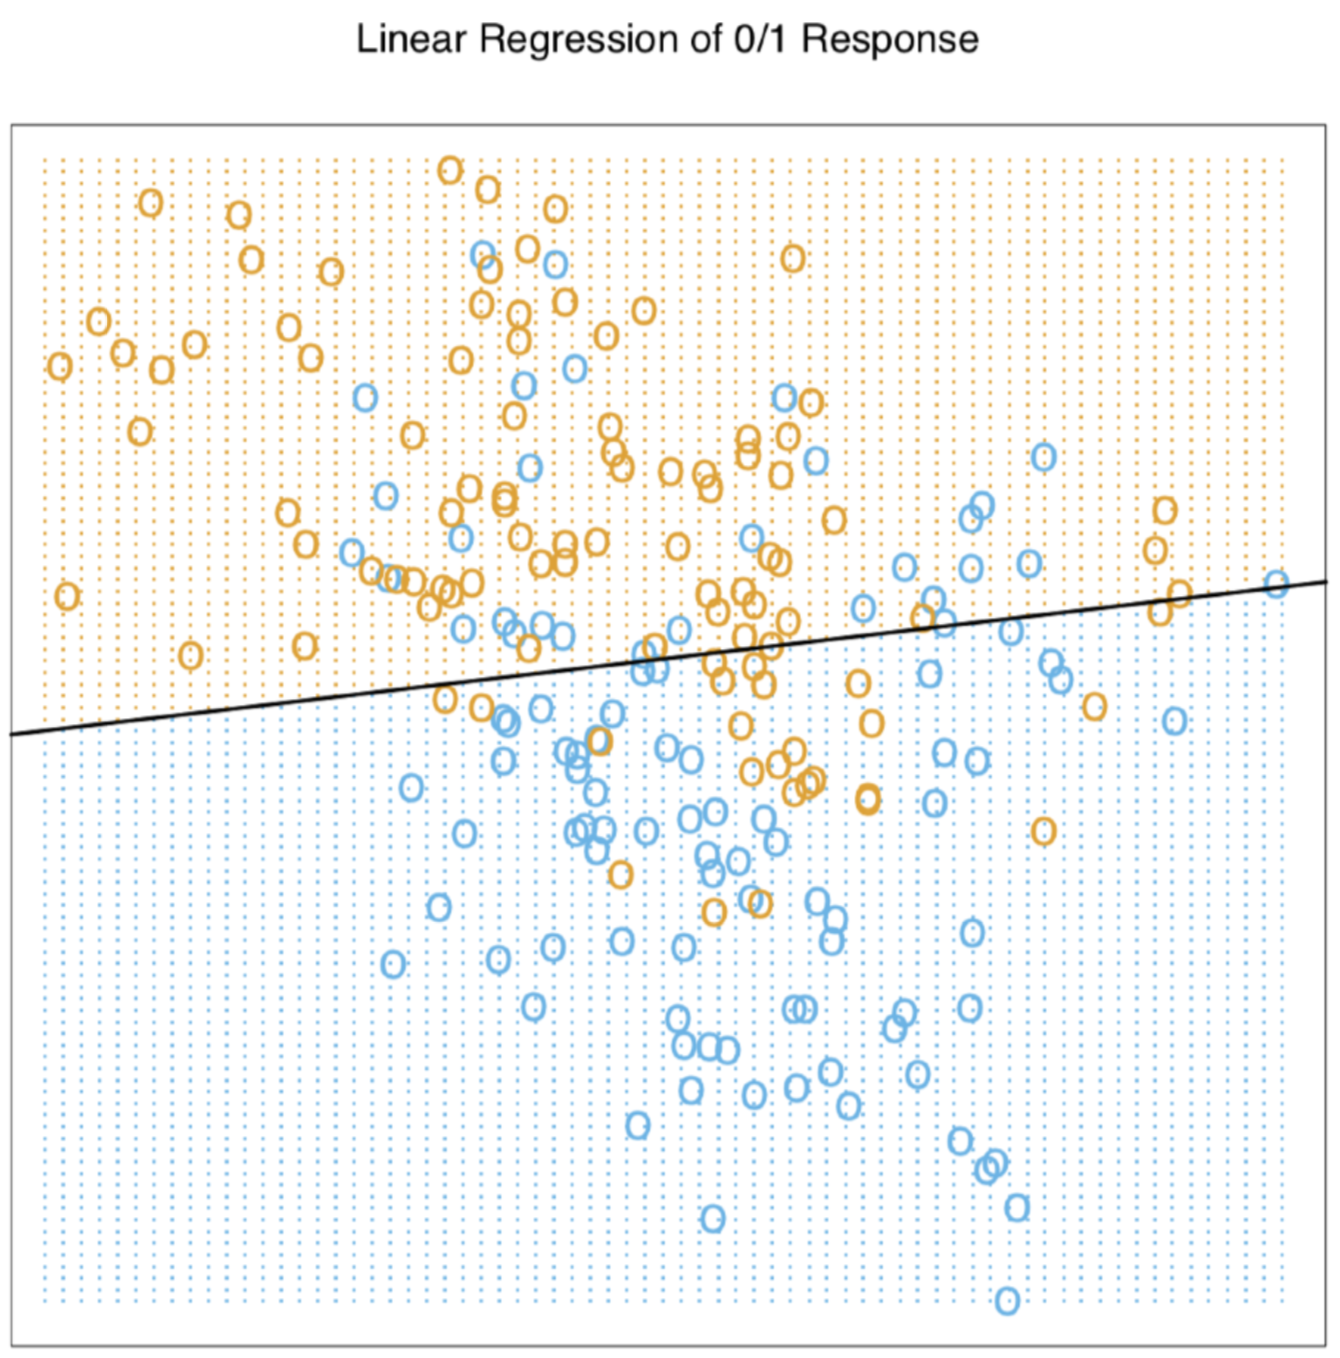
\includegraphics{./Figures/decboundary2D1.png}
    \caption{A classification example in two dimensions. The classes are coded
        as a binary variable (blue = 0, orange = 1), and then fit by linear
        regression. The line is the decision boundary, defined by
        $x^T \hat \beta = \half$ drawn as a black line. The orange shaded region
        denotes that part of input space classified as orange ($k=1$), while the
        blue region is classified as blue ($k=0$).
    }
    \label{decboundary2D1}
\end{marginfigure}

This method works only if the data are linearly separable -- \ie if we can
separate them in two sets of data by an hyperplan, defining the decision
boundary. We can there define an error.

It is worth noting that among many, we cannot predict in advance which prediction
method would work, without looking at the data. In practical, no method would
separate perfectly the data. If we augment the dimension of the space, we can
consider other functions. For example, quadratic regression would usually give
better results than linear. However, the use of higher dimensions spaces may
present tradeoffs: if we add more parameters, the training error would be reduced
, but the variance may also rise.
The issue here is to find the correct level of compexity that can fit the data,
without overfitting it and that can be generalised.

Again we'll use a second class of methods. ability to solve different issues.
fig 8 for example (marginfigure)

If we add to these data another class, for example $y=0,1,2$. There is now no
classical order between the values and the linear regression cannot be computed
on the three sets in one time. We have to split the data between two classes and
to find two decisions boundaries that split the three classes.

This was a very naive approach. Let's start again with $p=1$. Let's add more blue
squares at higher abscissa. This is presented in figure \ref{supvlearn7}


\begin{figure}
    \TODO
    \caption{Representation of a dataset with blue dots indexed as 0 and red
        dots indexed as 1. A linear regression can be plotted on these data
    }
    \label{supvlearn7}
\end{figure}

Here, we added data far enough to put the blue squares in another category.

The linear regression can be written as:

\begin{equation}
    \min_\beta \frac{1}{N} \sum_i (y_i - \beta x_i)^2
\end{equation}

We can see clearly that it is more convenient to work with more symmetric data.
Here we can define the error $\varepsilon_i$ for the $i$ index.

\begin{equation}
    \varepsilon_i = (y_i - \beta x_i)^2.
\end{equation}

For the $K=2$ problem, we can pose:

$k_i = \pm 1 bd$ if $\hat \beta x >0 => +1$
$if \hat \beta x<0 => -1$

What matters here is wether the quantity $\hat y = \hat \beta x$ has the correct
sign or not.

\begin{equation}
    L(\beta) = \frac{1}{N} \sum_i \max(0, -y_i\beta^T x_i)
\end{equation}

Here again, the idea is that when $\beta x$ is of the same sign as $y$, the
maximum is zero, and the error is zero. This is called hinge regression.

The idea of the problem is gradient descent, that as a smoother version, called
logistic regression.

the idea is to replace this version
fig 10.
\begin{equation}
    L(\beta) = \nth \sumin \ln (1+e^{-y_i \beta^T x_i} )
\end{equation}

he tries to minimise the error, and the split value with  that logistic regression.

we can also arrive to similar results by chosing different approaches.
this is connected to the kind of operations that are done in neural networks.
we will see this later on.

instead of taking the reflection y to be k, it's easier to consider y to be
a probability. it makes here much more sense to make a linear regression.
a probabilistic model, in which I want to describe the probability, given some data.
parameter $\omega$: weight, standard notation in neural networks, whereas $\beta$ is
much more used in classical regression/statistical learning models.

\begin{equation}
    P(k=1 | x,\omega)
\end{equation}

\begin{eqnarray}
    P(k=1|x,\omega ) & >  P(k=-1|x,\omega) & => \hat k = 1 \\
    & <      &  => \hat k = -1
\end{eqnarray}


if we are considering the log of the proabilities:
\begin{eqnarray}
    \ln \frac{P(k=1|x,\omega)}{P(k=-1|x,\omega)} & = & \omega^T x\\
    & = &  \sum_{j=1}^P \omega_j x_j (+\omega_0)
\end{eqnarray}


I don't have to always write $+\omega_0$, for convenience, just changes in the
problem that have no influence.

In general, I want to define a more relevant model.

Let's call:
\begin{equation}
    y=P(k=1|x,\omega)
\end{equation}
\begin{equation}
    \ln (\frac{y}{1-y}) = \omega^T x
\end{equation}

\begin{equation}
    \frac{y}{1-y} = \exp (\omega^T x)
\end{equation}

thus
\begin{equation}
    y = e^{\omega^T x} (1-y)
\end{equation}

therefore
\begin{equation}
    y(1+e^{\omega^T x}) = e^{\omega^T x}
\end{equation}

\begin{equation}
    y = \frac{e^{\omega^T x}}{1+e^{\omega^Tx}} = \frac{1}{1+e^{-\omega^T x}}
\end{equation}

\begin{equation}
    P(k|x,\omega) = \frac{1}{1+e^{-k\omega^T x}}
\end{equation}


\begin{equation}
    \mathcal{L}(\omega) = \frac{1}{N} \sum_i \ln P(k_i |x_i,\omega) MLE
\end{equation}

if i replace P by its form:

\begin{equation}
    \mathcal{L}(\omega) = - \frac{1}{N} \sum_i \ln (1 + e^{-k_i \omega^T x_i})
\end{equation}

Essentially, the idea was to apply the maximum likelihood. I had to make 
hypothesis on the general form of the model. Once I do this, I
end up with this function. The different with the one above:  minus sign.
not surprising: a likelihood we want to maximise, and not error we want to
minimize.

\begin{equation}
    \max_\omega \mathcal{L}(\omega) <=> \min_\beta L(\beta)
\end{equation}

in neural networks,

fig11

\begin{equation}
    u = \sum_{j=1}^p \omega_j x_j = \omega^T x 
\end{equation}
is called the activation.

several inputs, and one output based on this.
if $u>0$, then I have output $y=1$.
if $u<0$, then $y=0$.

in the context of neural networks, people prefer work with 0 and 1 rather than
$\pm 1$.

neuron is a classifier

fig11

\begin{equation}
    y = \phi (u)
\end{equation}

\begin{equation}
    \phi (u) = \frac{1}{1+e^{-u}}
\end{equation}

essentially, what we do, is considering the different inputs with different
weights.
At the end, we will end with more complex classifier models. this one is very
elementary.
there are very simple algorithms, like the gradient descent.


let's start again with the log likelihood:

\begin{eqnarray}
    \mathcal{L}(\omega) & = & \frac{1}{N} \sum_i (k_i \ln y_i + (1-k_i) \ln(1-y_i))\\
    & = & \frac{1}{N} \sum_i \ln P (k_i | x_i,\omega)
\end{eqnarray}

\begin{equation}
    y_i = P(k_i =1 |x,\omega)
\end{equation}

\begin{eqnarray}
    ln(P(\ldots)) & = y_i & \;\text{if}\; k_i = 1 \\
    & = 1-y_i & \;\text{if}\; k_i = 0
\end{eqnarray}

then we make the model by assuming:

\begin{equation}
    y_i = \phi (u_i) where u_i = \omega^T x_i = \sum_{j=1} \omega_j x_{ij}
\end{equation}

now, we want to compute the gradient.
it means to compute the derivative of the log likelihood:

\begin{equation}
    \frac{\partial \mathcal{L}}{\partial \omega_j} = \frac{1}{N} \sum_i (k_i \frac{1}{y_i} \frac{\partial y_i}{\partial\omega_j} - (1-k_i)
\frac{1}{1-y_i}) \frac{\partial y_i}{\partial \omega_j}
\end{equation}

with
\begin{equation}
    (\ldots) = \frac{ k_i (1-y_i) - (1-k_i)y_i}{y_i (1-y_i)} = \frac{k_i - y_i}{y_i (1-y_i)} 
\end{equation}


and \begin{equation}
    \frac{\partial y_i}{\partial \omega_j} = \phi'(u_i) \frac{\partial u_i}{\partial \omega_j} = \phi'(u_i) X_{ij}
\end{equation}


thus
\begin{equation}
    \frac{\partial \mathcal{L}}{\partial\omega_j} = \frac{1}{N} \sum_i \frac{\phi'(u_i)}{\phi(u_i) (1-\phi(u_i))} (k_i - y_i) x_{ij}
\end{equation}

\begin{equation}
    \phi (u) = \frac{1}{1+e^{-u}} => \frac{\phi''}{\phi (1-\phi)} = 1
\end{equation}

\begin{equation}
    \frac{\partial \mathcal{L}}{\partial \omega_j} = \frac{1}{N} \sum_i (k_i - y_i) x_{ij}
\end{equation}

for neural networks, the same idea as gradinet descent is called backpropagation
, but it is a bit more complicated.

fig 2.1: representation of classification.

support vector machine : SVM
problem formally attitred: 
\begin{equation}
    \min_\omega \sum_i \max(0,1-k_i \omega^T x_i ) + \lambda ||\omega||^2
\end{equation}

the exercise is trying to find what this function is doing.

standard linear regression: take care about the distance to the line.
when doing SVM: introducing some margin of errors.
this approach would count as an error even if we are on the right side of the
line but close to it.
we're not going to explain it here, but it looks very much linke the other frameworks.

another approach:
linear discriminant analysis (LDA)

we take a model (probabilistic), more gaussian like. the objective function is
to fit two classes by the gaussian, in such a way we maximise the distance
between the gaussians, and minimise the variance of the gaussians.
that can easily be done with linear algebra.

there are many other methods on the same lines.

Now we want to be able to adress the problem of non linear separability.
where the real boundary would be a circle.
in and out.

fig12

we can also do this locally.

it is called k-nearest neighbours

again, let's start with a batch of values:
fig13

we are given with a particular point, and say if it is red or blue.
what are the neighbours doing?

if $k=3$, i am looking at the three nearest points, and then take the colour of
the majority.

mathematically, it can be written as:

\begin{equation}
    \hat y(x)  = \frac{1}{k} \sum_{i\in N_k(x)} y_i
\end{equation}


$N_k(x)$ is the set of $k$ nearest neighbours to $x$

$y_i \in \{0,1\}$

Again, we can be in a situation described by fig 14.
we have, there, a decision boundary. i'm deciding what is the coulour of the
nearest points with that boundary.

fig 2.2 and 2.3. variations of K

now the question is: what should we take for K

$\frac{N}{k} \sim p$ : number of degrees of freedom.


fig 15

figure slide: 'selection of K': using 10,000 datapoints and tested with 200.

minimal training error if we take k=1. very complicated thing.
as we are taking larger and larger values of k, we are averaging and get more
errors, even in the training set.
if we have too few degrees of freedom, we are completely missing the structure
of data.
it is also not good if we have too many degrees of freedom.

15 is relatively well located in this area.
between 20 and 10, there's not that much difference, maybe 10 is better
because it uses less resources.
we have to pick the right model, and there are models of different levels of
complexity.
different values of k that can be used.

there is nothing into this algorithm, but also nothing trivial in finding the right datapoints.

there are many variations along this method.
in this example, we are taking the same density of points, everywhere. but if I take any point, it doesn't mean anything to take just three points
randomly.
we may take into account the distance between the points.
essentially, we would average around the point that are close to the considered
point. more generally, we can do it with a hard cutoff close/far or smooth
cutoffs.

\begin{equation}
    \hat y(x) = \frac{\sum_i K_\lambda (x,x_i)y_i}{\sum_i k_\lambda (x,x_i)}
\end{equation}

\begin{equation}
    K_\lambda (x,x_i) = \frac{1}{\lambda} e^{-\frac{||x-x'||^2}{2\lambda}}
\end{equation}

or $K_\lambda (x,x_i) = 1$ if $||x-x'||<\lambda$, 0 otherwise.

kernel methods also posisble.
if we do this, it is also a case where we have one parameter: $\lambda$. It plays
the same role.
big lambda: averaging a lot.
we would reduce the variance, but with a too large bias.
in the opposite: reduce the bias would end in a too large variance.

again, there are variety of methods that can be used. one way to see this
problem of classification is to fit a function.
let's say, zero for orange points, 1 for blue points.

At one dimension, we would have
fig 16.

maybe there could be errorsa

the thing is that we may smooth all those functinos.
we may think about these problems as fitting problems. correcting locally
the errors of the functions.

kernel method smoothing, to locally have something smoother.
what these things are doing is similar to the problem of smoothly inferring a
function from just any perfect observation.

This is very simple, but the problem is that none of those things are working
for big data. issue of classifying dogs and cats.

If we go in any of those methods, there is no way we can succeed. Several
problems, the greatest is a geometrical one:
the curse of dimensionality.

essentially, it has to do with all the assumption we have about neighbourhoods
are false when we are working with high dimensional spaces.

example in 2D in fig 17.

volume is scaling as power p of the radius. $V = \alpha_p r^p$.

If we look at $\frac{V}{V_{tot}} = \left( \frac{r}{r_{tot}} \right)^p$

then we have 

\begin{equation}
    \frac{r}{r_{tot}} = \left( \frac{V}{V_{tot}} \right)^{1/p}
\end{equation}


If the ratio $\frac{V}{V_{tot}} = 0.01$.
if we take something like p=10, we'll see that $\frac{r}{r_{tot}} = 0.6$.

if we want to cover even a very small fraction of the volume, we have to go very
far from the point.
ridiculous amount of the volume.
the problem of scaling with the radius is not interesting.
in high dimensional spaces, all the volume is close to the centre.

to cover a small fraction of the volume, we have to go very far.

All the ideas of closest neighhbourgs cannot be used in high dimensionality
spaces.

we can also reduce the dimensionality of the data. that is the first approach
with this problem.
solutions:
\begin{itemize}
    \item reduce dimensionality -> PCA (unsupervised)
    \item representation, that has to do with what kind of space we are woking with. we have to imagine that we have all the pictures of cats and
        dogs, all put in the same place.
        something invariant with translation, rotation, etc. so this will be seen in another lecture, about neural networks. essentially, one
        class of netwkrs: convolutional, is based on this. chose the right space
        in which it is easy to chose the classification.
\end{itemize}

exam
In priciple, everything should be comprised in the lecture.
code it ourself. not using things already written. the game here is to write
ourself our own libraries. it is not very complicated, each question is just
a few lines of code.

with python: using the jupyter.
matlab: not sure it is doeable. livescripts.
write a report in which he can see the code. in a format he can actually work
the code.
minimal thing: write the code and display the figures.
this is a public problem, neither on the solutions presented on the internet is
good, we might think about it from ourselves.





